\chapter{Architettura del Sistema}\label{chap:third}

\inlineminitoc

In questo capitolo viene presentata l'architettura complessiva del sistema sviluppato, illustrando i componenti principali e il flusso di dati attraverso le diverse fasi del processo. L'obiettivo è fornire una panoramica chiara e dettagliata delle scelte progettuali, tracciando il percorso logico che i dati seguono dal momento in cui vengono acquisiti fino alla fase di interrogazione e utilizzo da parte degli utenti finali.

La Figura \ref{fig:architettura-software} fornisce un diagramma riassuntivo di tale architettura, evidenziando i moduli principali e le interazioni tra di essi. Come illustrato nello schema, il sistema è concepito come una pipeline sequenziale. 

Nella prima fase, vengono applicate tecniche specifiche per il recupero dei testi grezzi dai documenti normativi, con particolare attenzione alle librerie impiegate per il parsing e alle strategie di pulizia dei dati, fondamentali per mitigare rumore e inconsistenze strutturali.

Una volta estratto, il testo necessita di essere organizzato secondo le logiche giuridiche del documento. A tale scopo, la fase di strutturazione si avvale di Large Language Models (LLM) per la trasformazione del testo grezzo in un formato analizzabile. Il fulcro di questo passaggio è la definizione e l'utilizzo di uno schema JSON rigoroso, progettato appositamente per rappresentare e mantenere intatta la gerarchia degli atti normativi e le complesse relazioni giuridico-logiche che li collegano.

I dati validati e strutturati vengono successivamente indirizzati verso il sistema di archiviazione, cioè il database Neo4j, che inserisce le informazioni mantenendo le relazioni gerarchiche e logiche tra i vari elementi normativi precedentemente individuati.

Dopodiché vengono calcolati gli \textit{embedding} testuali a partire dal testo dei commi, informazione presente come proprietà del nodo. Questi \textit{embedding} vengono memorizzati nel database, consentendo di effettuare ricerche basate sulla similarità semantica.

Infine viene effettuato un confronto architetturale e prestazionale tra due diversi paradigmi di ricerca:

\begin{itemize}
    \item L'implementazione di una \textbf{ricerca vettoriale classica} basata puramente sulla \textit{cosine similarity}. Sfruttando le rappresentazioni vettoriali archiviate, questo approccio è mirato a simulare la ricerca per similarità in un ambiente vettoriale puro, fungendo così da termine di paragone fondamentale per la successiva fase di benchmarking tra l'interrogazione puramente semantica e quella arricchita dalla struttura a grafo.
    \item L'implementazione di una \textbf{ricerca ibrida (vettoriale e strutturale)}, in cui il calcolo della similarità semantica viene arricchito dalla topologia del grafo. In questa configurazione, il database non si limita a ospitare gli \textit{embedding} testuali, ma sfrutta le relazioni gerarchiche, sequenziali e logiche del corpus normativo. Questo approccio permette di combinare il recupero dell'informazione semantica con il contesto relazionale fornito dalla struttura del documento.
\end{itemize}

\begin{figure}[H]
    \centering
    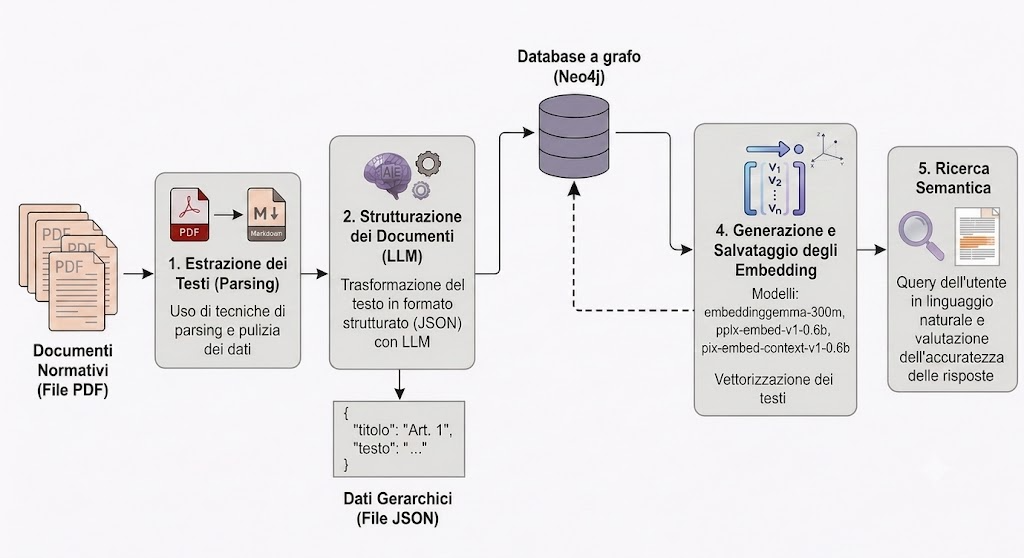
\includegraphics[width=1\textwidth]{_images/architettura-software.png}
    \caption{Architettura del sistema}
    \label{fig:architettura-software}
\end{figure}